
%+PATCH,//BRILL/TEX
%+DECK,getting_started,T=LATEX.

\renewcommand*\thesection{\Roman{section}}
\section{Getting Started}

First, we open a terminal and clone the whole package from Github to the directory
\bri:

\cbox{git clone https://github.com/MicScheer/brill.git brill}

We call the directory \bri of \pB it's home directory and the
sub-directory \sta the working directory.

Since \urp is a standalone program, we can run it by hand, i.e. not
deploying \pBe. We change to the \wdir and run \urpe:

\cbox{
cd stage\\
../bin/urad\_phase.exe
}

The program should run and write some lines to the terminal.\\

\begin{figure}[htb]
   \centering
   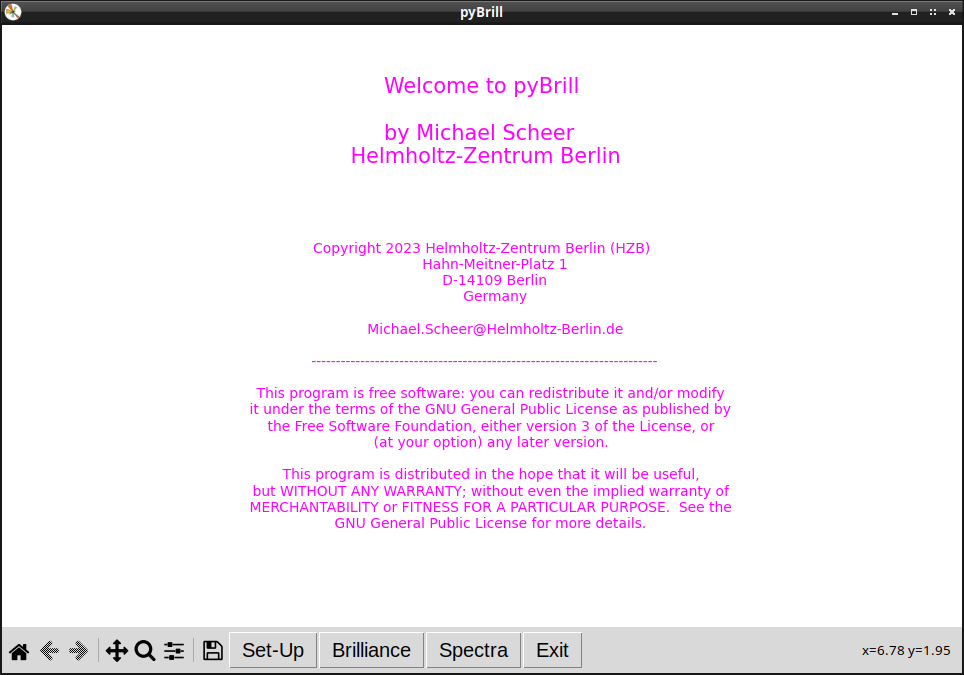
\includegraphics[width=0.8\textwidth]
   {pictures/pybrill.png}
   \caption{Start Menu of pyBrill}
   \label{gsfig1}
\end{figure}
		
\Urp reads the input data from a namelist file \uname. This file can
be edit by the user, but it also can be created by \pBe, which has
menus to set the variables, run \urpe, and plots the results.

We start \pB and try it:\\[-1.0cm]

\cbox{
python3 -i ../python/pyBrill.py
}

The size and position of the window can be controlled by editing the
first line of\\[-1.0cm]

\cbox{
ntupplot.cfg
}

The other parameters are not relevant for \pBe. An example of this file can be found
in the sub-directory \git{input} of the home directory of \pBe.

\subsection{Brilliance Calculations}

\begin{figure}[htb]
   \centering
   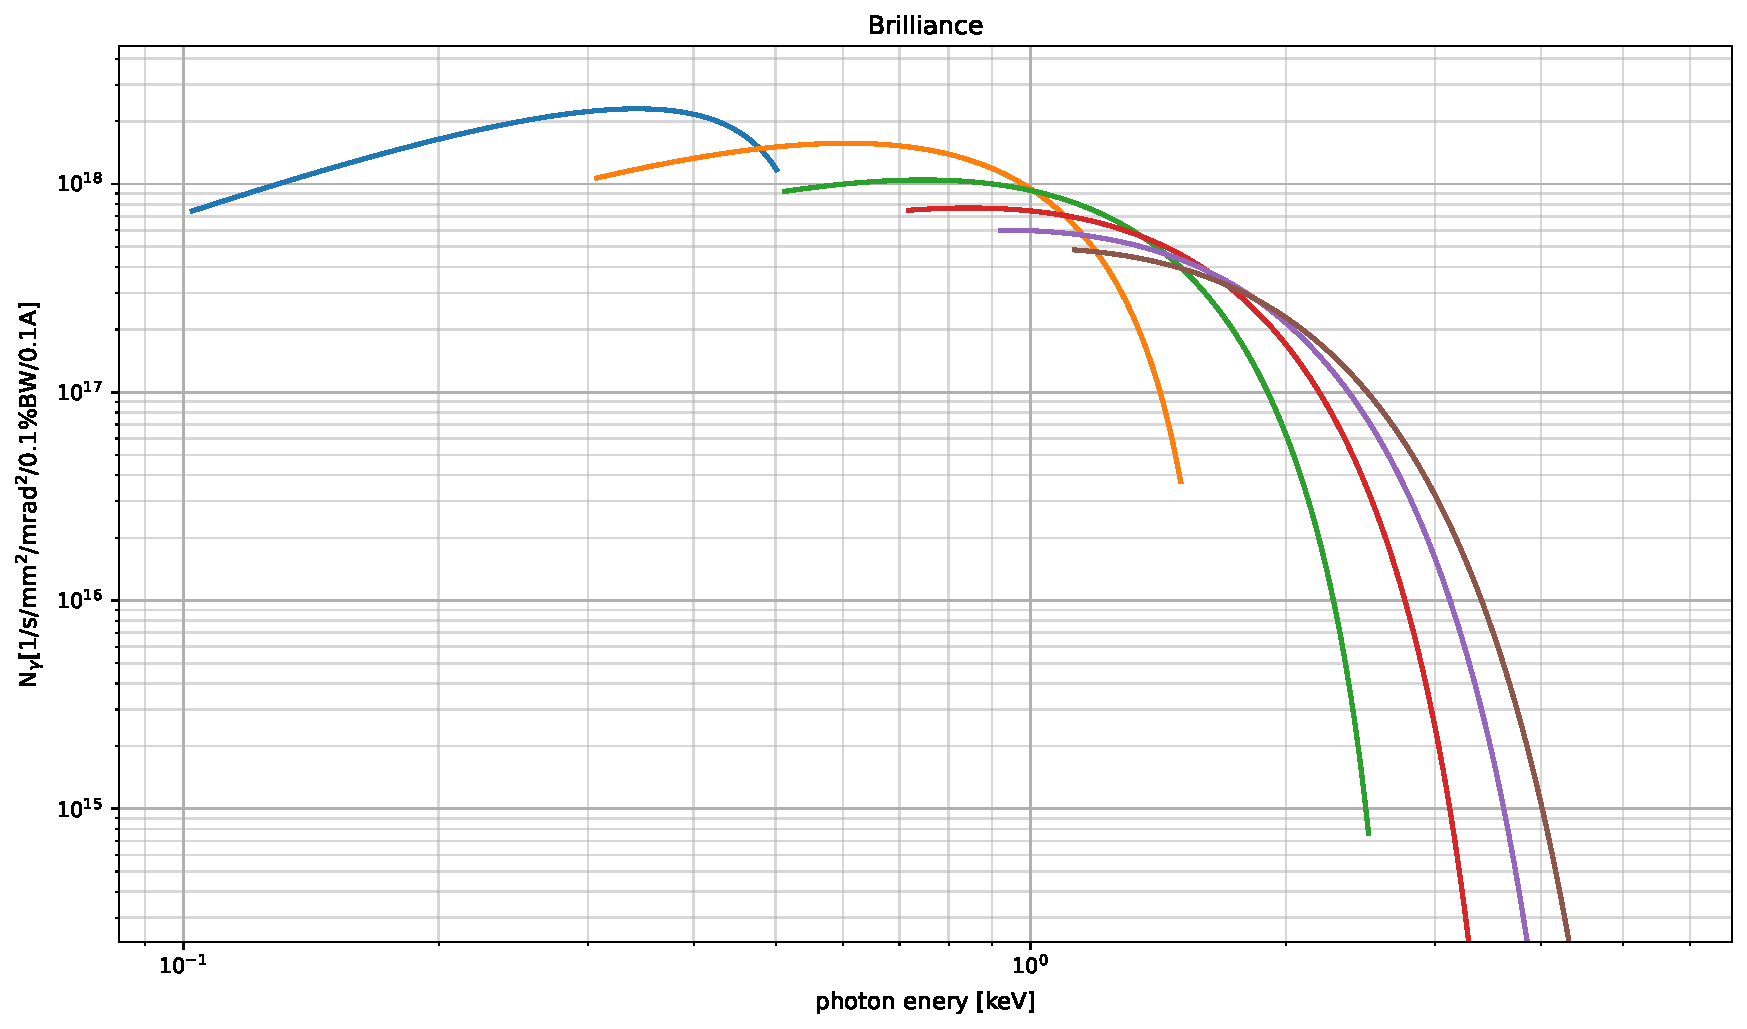
\includegraphics[width=0.8\textwidth]
   {pictures/brilliance.pdf}
   \caption{Brilliance Plot}
   \label{gsfig2}
\end{figure}

Press the button labeled \git{Brilliance} and plot the brilliance of the
undulator. As you can see in the terminal, the plotted data are
written to files. The plot itself is save as PDF-file.

To control the brilliance calculation, press the \gti{Set-Up} button
and check the menu items. The \gti{spectra} item is not used the
brilliance calculations. It is reserved for the spectra calculations
with \urpe.

The default values are set by \pB or read from a file named

\cbox{.pybrill\_last.dat}

which is written when the \gti{Exit} button of \pB is pressed. Note,
if you leave \pB by entering "q" while the focus is on the output
screen, the data are not stored.

\subsection{Spectrum Calculations}

\begin{figure}[htb]
   \centering
   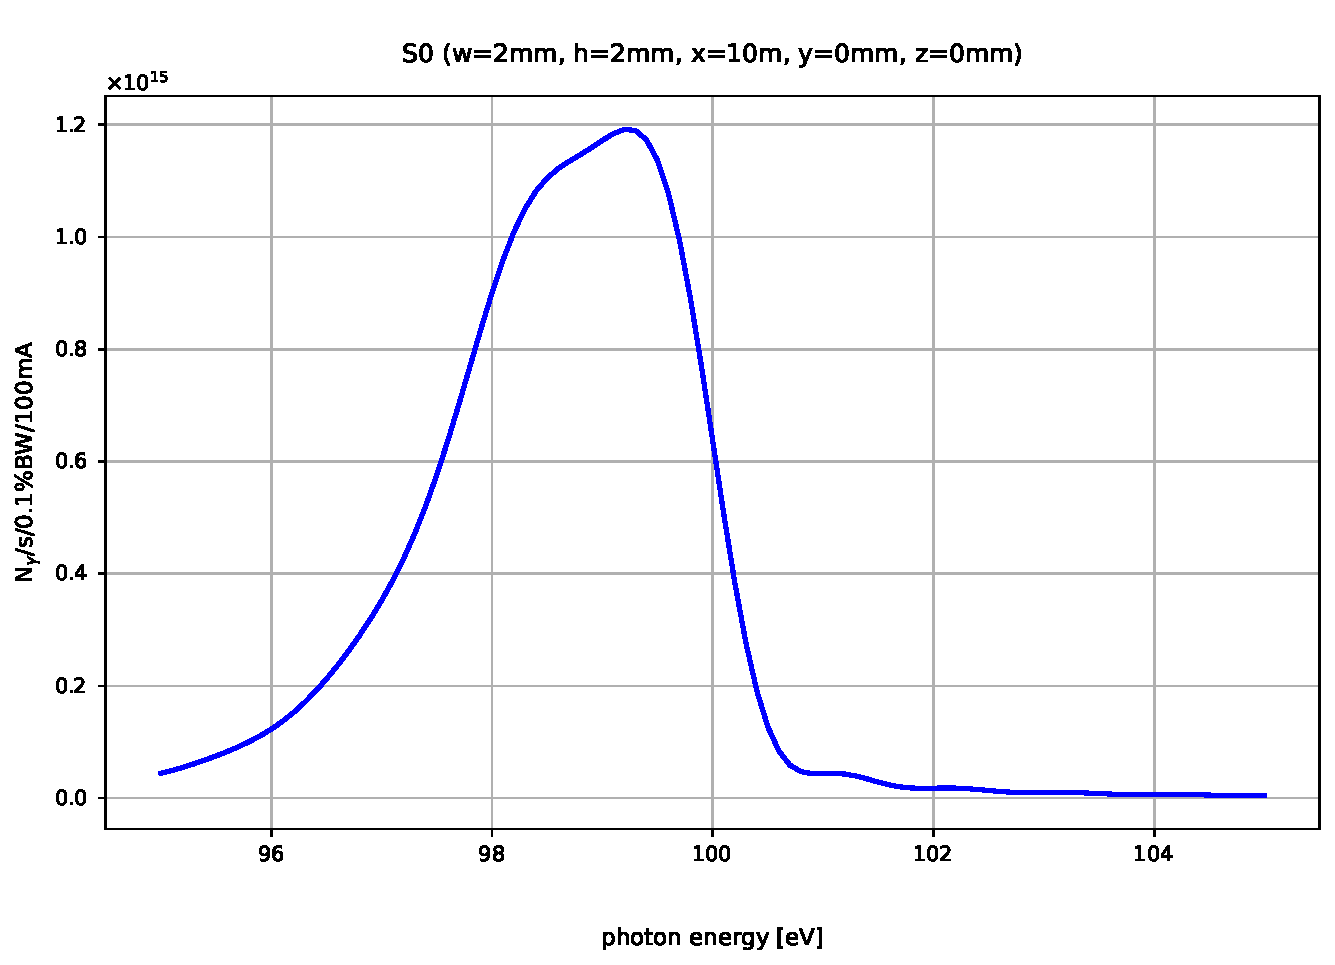
\includegraphics[width=0.7\textwidth]
   {pictures/flux.pdf}
   \caption{Flux of Undulator}
   \label{gsfig3}
\end{figure}

Press the \gti{Spectra} button, select \gite{Plot/Flux/Stokes/S0}. The
flux of the Stokes parameter \git{S0} through the rectangular pinhole
as calculated by \urp is plotted (Fig. \ref{gsfig3}).

\begin{figure}[htb]
   \centering
   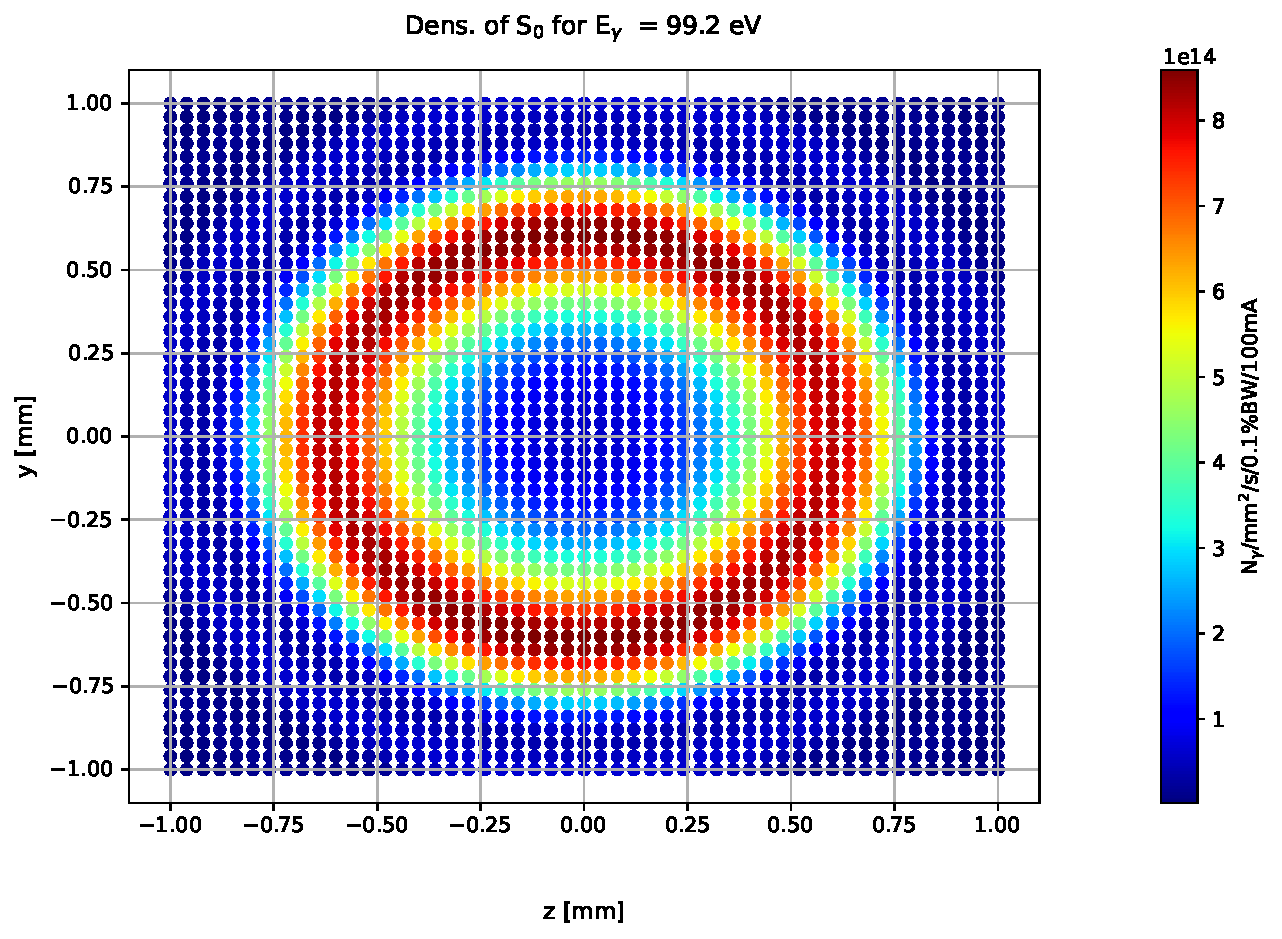
\includegraphics[width=0.7\textwidth]
   {pictures/fdpin.pdf}
   \caption{Flux-density Distribution}
   \label{gsfig4}
\end{figure}

Now, we select
\gti{Spectra/Plot/Distributions in Pinhole/Stokes/S0}
and see the flux-density distribution of \gti{S0}. The photon energy is
selected to show the distribution for the photon energy which the
maximum flux trough the pinhole.

To step through the photon energies, the arrows of the keyboard can be
used. The photon energy can also be selected from the menu

\cbox{\gti{Spectra/Plot/Distributions in Pinhole/Select E\_photon}
}

